\section{Beispiel Datensatz}
\label{id3:datensatz}
Zur Veranschaulichung des ID3 Algorithmus wurde ein Datensatz \textit{S} gewählt welcher in Tabelle \ref{table:datensatz-original} dargestellt ist. \Autocite{ImplementationID3}. Dieser Datensatz beinhaltet die Attribute \textit{WEATHER}, \textit{TEMP}, \textit{HUMIDITY} und \textit{WIND} sowie ein Klassifizierung \textit{PLAY}.\\
Hierbei ist die Aufgabe den ID3 Allgorithmus zu nutzen um einen Entscheidungsbaum zu erstellen um vorherzusagen ob das Wetter ermöglicht dass Fußball gespielt werden kann.

\begin{table}[htbp]
    \centering
    \begin{tabular}{cccccc}
        \toprule
        \textbf{DAY} & \textbf{WEATHER} & \textbf{TEMP} & \textbf{HUMIDITY} & \textbf{WIND} & \textbf{PLAY} \\
        \toprule
        1   &Sunny	&Hot	&High	&Weak	&No  \\
        2   &Sunny	&Hot	&High	&Strong	&No  \\
        3   &Cloudy	&Hot	&High	&Weak	&Yes \\
        4   &Rainy	&Medium	&High	&Weak	&Yes \\
        5   &Rainy	&Cold	&Normal	&Weak	&Yes \\
        6   &Rainy	&Cold	&Normal	&Strong	&No  \\
        7   &Cloudy	&Cold	&Normal	&Strong	&Yes \\
        8   &Sunny	&Medium	&High	&Weak	&No  \\
        9   &Sunny	&Cold	&Normal	&Weak	&Yes \\
        10  &Rainy	&Medium	&Normal	&Weak	&Yes \\
        11  &Sunny	&Medium	&Normal	&Strong	&Yes \\
        12  &Cloudy	&Medium	&High	&Strong	&Yes \\
        13  &Cloudy	&Hot	&Normal	&Weak	&Yes \\
        14  &Rainy	&Medium	&High	&Strong	&No  \\
        \bottomrule
    \end{tabular}
    \caption{Beispiel Datensatz \textit{S}}
    \label{table:datensatz-original}
\end{table}

Als erstes werden die Informationsgewinne für die Attribute aus dem Datensatz \textit{S} berechnet. Dabei ergibt sich folgende Übersicht.

\begin{table}[htbp]
    \centering
    \begin{tabular}{lc}
        \textit{IG}(\textit{S}, \textit{WEATHER})  &= 0.246749 \\
        \textit{IG}(\textit{S}, \textit{TEMP})     &= 0.029222 \\
        \textit{IG}(\textit{S}, \textit{HUMIDITY}) &= 0.151835 \\
        \textit{IG}(\textit{S}, \textit{WIND})     &= 0.048127 \\
    \end{tabular}
\end{table}

Da das Attribut \textit{WEATHER} den höchsten Informationsgewinn hat wird es als Knoten bzw. Wurzelknoten gewählt. \textit{WEATHER} besitzt die drei möglichen Ausprägungen \textit{Sunny}, \textit{Cloudy} und \textit{Rainy} für die nun im jeweiligen Iterationschritt eine Teilmenge von \textit{S} erzeugt wird. Daraus ergibt sich zunächst für die Ausprägung \textit{Sunny} folgende Teilmenge $S_{1} = S_{WEATHER=Sunny}$.

\begin{table}[H]
    \centering
    \begin{tabular}{cccccc}
        \toprule
        \textbf{DAY} & \textbf{WEATHER} & \textbf{TEMP} & \textbf{HUMIDITY} & \textbf{WIND} & \textbf{PLAY} \\
        \toprule
        1   &Sunny	&Hot	&High	&Weak	&No  \\
        2   &Sunny	&Hot	&High	&Strong	&No  \\
        8   &Sunny	&Medium	&High	&Weak	&No  \\
        9   &Sunny	&Cold	&Normal	&Weak	&Yes \\
        11  &Sunny	&Medium	&Normal	&Strong	&Yes \\
        \bottomrule
    \end{tabular}
    \caption{Teilmenge $S_{1}$}
    \label{table:datensatz-sunny}
\end{table}

Für $S_{1}$ wird nun rekursiv ein Teilbaum erzeugt wobei die Teilmenge keine der Abbruchbedingungen erfüllt, sodass man nun mit der Berechnung der Informationsgewinne für die Attribute aus $S_{1}$ fortfahren kann. Dabei ergeben sich folgende Werte.

\begin{table}[htbp]
    \centering
    \begin{tabular}{lc}
        \textit{IG}(\textit{S}, \textit{TEMP})     &= 0.570951 \\
        \textit{IG}(\textit{S}, \textit{HUMIDITY}) &= 0.970951 \\
        \textit{IG}(\textit{S}, \textit{WIND})     &= 0.019973 \\
    \end{tabular}
\end{table}

Nun wird das Attribut \textit{HUMIDITY} als Knoten gewählt da es nun den höchsten Informationsgewinn besitzt. Dabei hat \textit{HUMIDITY} die zwei mögliche Ausprägungen \textit{High} und \textit{Normal}. Somit ergeben sich die Teilmengen $S_{1_{HUMIDITY=High}}$ und $S_{1_{HUMIDITY=Normal}}$ aus $S_{1}$.

\begin{table}[H]
    \centering
    \begin{tabular}{cccccc}
        \toprule
        \textbf{DAY} & \textbf{WEATHER} & \textbf{TEMP} & \textbf{HUMIDITY} & \textbf{WIND} & \textbf{PLAY} \\
        \toprule
        1   &Sunny	&Hot	&High	&Weak	&No  \\
        2   &Sunny	&Hot	&High	&Strong	&No  \\
        8   &Sunny	&Medium	&High	&Weak	&No  \\
        \bottomrule
    \end{tabular}
    \caption{Teilmenge $S_{1_{HUMIDITY=High}}$}
    \label{table:datensatz-humidity-high}
\end{table}
\begin{table}[H]
    \centering
    \begin{tabular}{cccccc}
        \toprule
        \textbf{DAY} & \textbf{WEATHER} & \textbf{TEMP} & \textbf{HUMIDITY} & \textbf{WIND} & \textbf{PLAY} \\
        \toprule
        9   &Sunny	&Cold	&Normal	&Weak	&Yes \\
        11  &Sunny	&Medium	&Normal	&Strong	&Yes \\
        \bottomrule
    \end{tabular}
    \caption{Teilmenge $S_{1_{HUMIDITY=Normal}}$}
    \label{table:datensatz-humidity-normal}
\end{table}

Betrachtet man oben genannten Teilmengen fällt sofort auf dass alle Objekte dieser Teilmengen die jeweils die selbe Klassifizierung besitzen. Für $S_{1_{HUMIDITY=High}}$ nämlich die Klassifizierung \textit{No} und für $S_{1_{HUMIDITY=Normal}}$ die Klassifizierung \textit{Yes}. Daher wird für beide Ausprägungen des Knotens \textit{Humidity} ein Blatt erstellt welches jeweils die entsprechende Klassifizierung zugewiesen bekommt. Daraus ergibt sich folgender vorläufiger Teilbaum.

\begin{figure}[htbp]
    \centering
    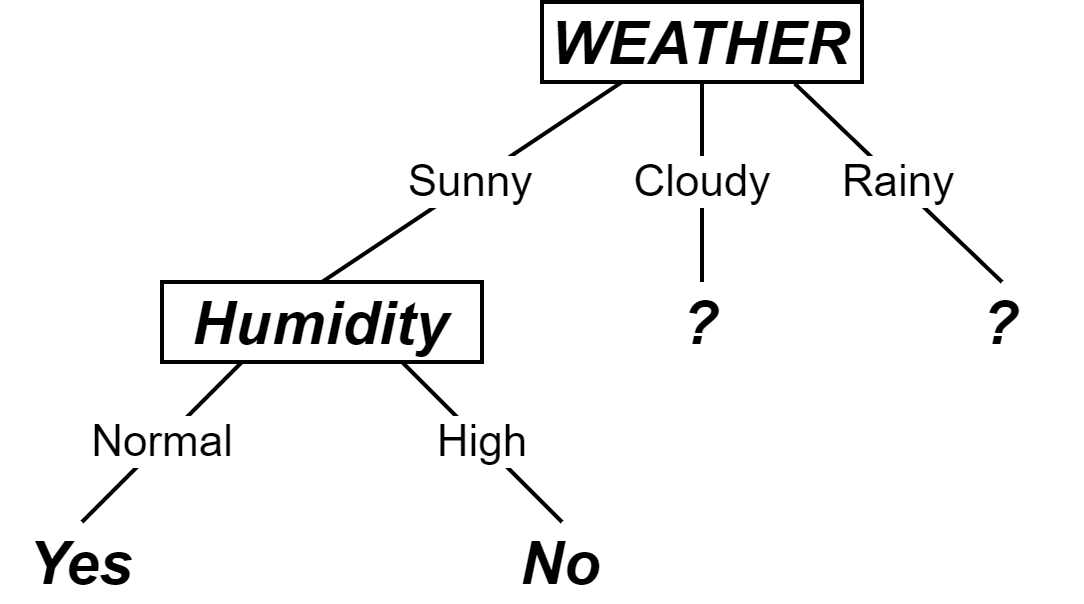
\includegraphics[width=.5\textwidth]{Subtree-Humidity.png}
    \caption{Vorläufiger Teilbaum nachdem \textit{HUMIDITY} klassifiziert wurde}
\end{figure}

Da nun die Ausprägungen des Attributes \textit{HUMIDITY} klassifiziert worden sind fahren wir mit der zweiten Ausprägung von \textit{WEATHER} fort, nämlich \textit{Rainy}. Für diese wird die Teilmenge $S_{2} = S_{WEATHER=Rainy}$ erstellt.

\begin{table}[htbp]
    \centering
    \begin{tabular}{cccccc}
        \toprule
        \textbf{DAY} & \textbf{WEATHER} & \textbf{TEMP} & \textbf{HUMIDITY} & \textbf{WIND} & \textbf{PLAY} \\
        \toprule
        4   &Rainy	&Medium	&High	&Weak	&Yes \\
        5   &Rainy	&Cold	&Normal	&Weak	&Yes \\
        6   &Rainy	&Cold	&Normal	&Strong	&No  \\
        10  &Rainy	&Medium	&Normal	&Weak	&Yes \\
        14  &Rainy	&Medium	&High	&Strong	&No  \\
        \bottomrule
    \end{tabular}
    \caption{Teilmenge $S_{2}$}
    \label{table:datensatz-Rainy}
\end{table}

Für $S_{2}$ wird nun erneut der Informationsgewinn der verbleibenden Attribute berechnet. Zu diesem Zeitpunkt bleiben nur noch die Attribute \textit{TEMP} und \textit{WIND} übrig, da die anderen Attribute bereits verwendet worden sind. Es ergeben sich folgende Werte für den Informationsgewinn.

\begin{table}[htbp]
    \centering
    \begin{tabular}{lc}
        \textit{IG}(\textit{S}, \textit{TEMP})     &= 0.019973 \\
        \textit{IG}(\textit{S}, \textit{WIND})     &= 0.970951 \\
    \end{tabular}
\end{table}

Basierend auf den Informationsgewinnen wird \textit{WIND} als Knoten gewählt. Dieses Attribut besitzt die zwei Ausprägungen \textit{Weak} und \textit{Stong}. Somit ergeben sich die Teilmengen $S_{2_{WIND=Weak}}$ und $S_{2_{WIND=Strong}}$ aus $S_{2}$.

\begin{table}[H]
    \centering
    \begin{tabular}{cccccc}
        \toprule
        \textbf{DAY} & \textbf{WEATHER} & \textbf{TEMP} & \textbf{HUMIDITY} & \textbf{WIND} & \textbf{PLAY} \\
        \toprule
        4   &Rainy	&Medium	&High	&Weak	&Yes \\
        5   &Rainy	&Cold	&Normal	&Weak	&Yes \\
        10  &Rainy	&Medium	&Normal	&Weak	&Yes \\
        \bottomrule
    \end{tabular}
    \caption{Teilmenge $S_{2_{WIND=Weak}}$}
    \label{table:datensatz-wind-weak}
\end{table}

\begin{table}[H]
    \centering
    \begin{tabular}{cccccc}
        \toprule
        \textbf{DAY} & \textbf{WEATHER} & \textbf{TEMP} & \textbf{HUMIDITY} & \textbf{WIND} & \textbf{PLAY} \\
        \toprule
        6   &Rainy	&Cold	&Normal	&Strong	&No  \\
        14  &Rainy	&Medium	&High	&Strong	&No  \\
        \bottomrule
    \end{tabular}
    \caption{Teilmenge $S_{2_{WIND=Strong}}$}
    \label{table:datensatz-wind-strong}
\end{table}

Bei beiden Teilmengen fällt auf dass alle Objekte aus diesen Teilmengen die selbe Klassifizierung aufweisen. An dieser Stelle wird analog zum Vorgehen beim Attribut \textit{HUMIDITY} ein Blatt für die Ausprägungen von \textit{WIND} erstellt. Darus ergibt sich nun folgender Teilbaum.

\begin{figure}[htbp]
    \centering
    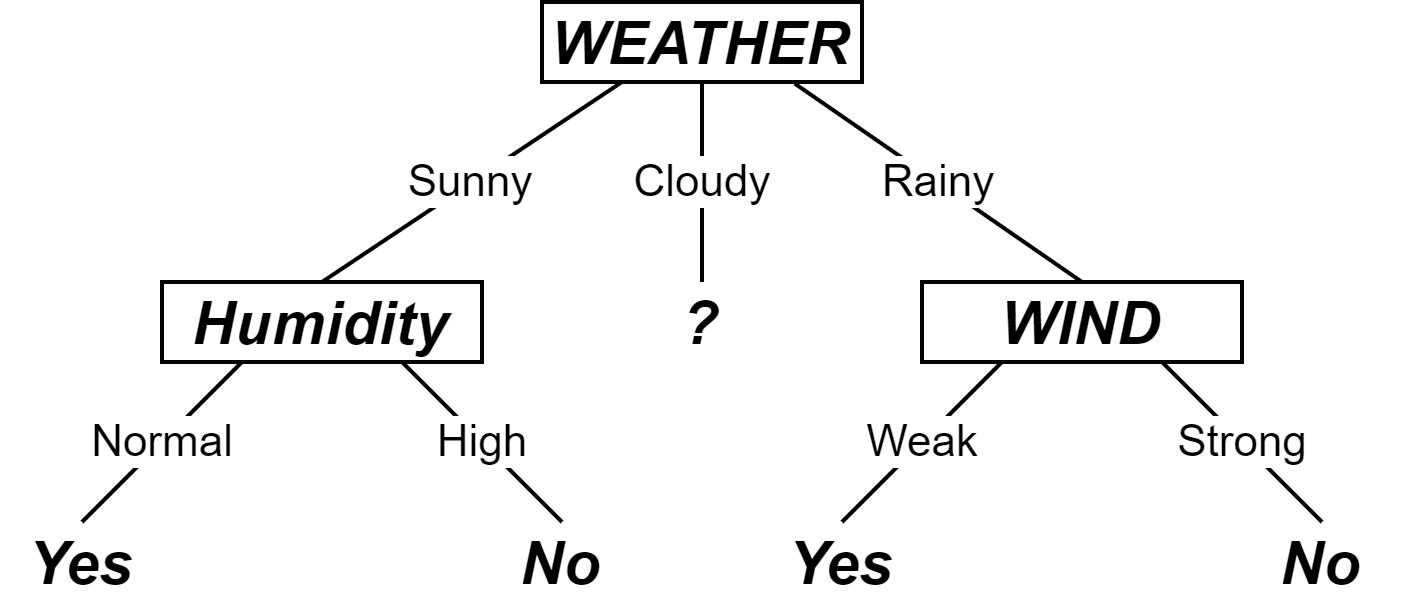
\includegraphics[width=.7\textwidth]{Subtree-Wind.png}
    \caption{Vorläufiger Teilbaum nachdem \textit{WIND} klassifiziert wurde}
\end{figure}

Nachdem also nun die Klassifizierung für das Attribut \textit{WIND} und somit auch für die Ausprägung \textit{Rainy} abgeschlossen ist, bleibt nur noch die Ausprägung \textit{Cloudy} zur Klassifizierung übrig. Basierend darauf ergibt sich folgende Teilmenge $S_{3} = S_{WEATHER=CLoudy}$.

\begin{table}[htbp]
    \centering
    \begin{tabular}{cccccc}
        \toprule
        \textbf{DAY} & \textbf{WEATHER} & \textbf{TEMP} & \textbf{HUMIDITY} & \textbf{WIND} & \textbf{PLAY} \\
        \toprule
        3   &Cloudy	&Hot	&High	&Weak	&Yes \\
        7   &Cloudy	&Cold	&Normal	&Strong	&Yes \\
        12  &Cloudy	&Medium	&High	&Strong	&Yes \\
        13  &Cloudy	&Hot	&Normal	&Weak	&Yes \\
        \bottomrule
    \end{tabular}
    \caption{Teilmenge $S_{3}$}
    \label{table:datensatz-cloudy}
\end{table}

Bei der Betrachtung von $S_{3}$ fällt auf dass alle beinhalteten Objekte die selbe Klassifizierung \textit{Yes} besitzen. Aus diesem Grund wird analog zu der Vorgehensweise bei \textit{WIND} und \textit{HUMIDITY} ein Blatt mit der entsprechenden Klassifizierung erstellt. Somit wird der ID3 Algorithmus beendet und es entsteht der folgende finale Entscheidungsbaum.

\begin{figure}[H]
    \centering
    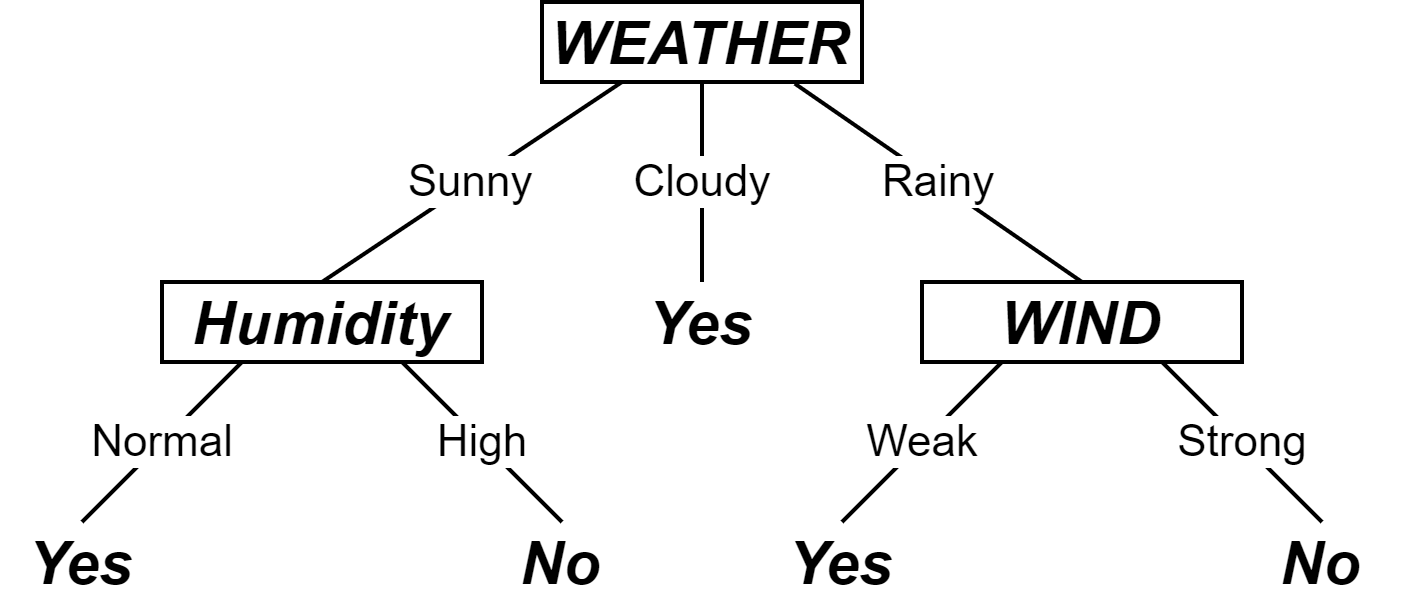
\includegraphics[width=.7\textwidth]{Subtree-Final.png}
    \caption{Finaler Entscheidungsbaum}
\end{figure}

Aus dem oben dargestellten Entscheidungsbaum ergeben sich folgende Regeln für das Spielen. 

\begin{enumerate}
    \item Wenn das Wetter sonnig ist und die Humidität normal, dann kann Fußball gespielt werden. Wenn die Humidität allerdings hoch ist, dann kann kein Fußball gespielt werden. \autocite{ImplementationID3}
    \item Wenn das Wetter bewölkt ist, dann kann Fußball gespielt werden. \autocite{ImplementationID3}
    \item Wenn das Wetter regnerisch ist und der Wind schwach, dann kann Fußball gespielt werden. Falls aber der Wind stark ist, dann kann kein Fußball gespielt werden. \autocite{ImplementationID3}
\end{enumerate}

\pagebreak